\chapter{Thermodynamik}
\section{Grundbegriffe der Thermodynamik}
\textbf{Energie E}\\
= Fähigkeit eines Systems Arbeit zu verrichten
\begin{itemize}
	\item kinet. E = $\frac{1}{2}*m*v^2$
	\item elektr. E = $U/d$
	\item pot. E = $m*g*h$
	\item Wärmeenergie = $m*c_p+\Delta T$ , wenn $p=const.$
	\item Photonenenergie = $h*f$
\end{itemize}

\textbf{Arbeit W}
\begin{itemize}
	\item mech. Arbeit = $F*s$
	\item elektr. Arbeit = $P*t=I^2*R*t$
	\item Volumenarbeit = $-p*\text{d}V$
\end{itemize}

\textbf{Leistung P} = $\frac{W}{t}$\\ \\

\textbf{\underline{Arten von Systemen:}}
\begin{itemize}
	\item \textbf{offenes System}: Energie und Stoff
	\item  \textbf{geschlossenes System}: Energie
	\item  \textbf{abgeschlossenes System}: nichts ("`adiabat"') 
\end{itemize}

\section{Ideales Gasgesetz}
\textbf{Satz von Avogadro}: \\
$V=\text{Konstante}*n$ für $T,p = const.$\\

\textbf{Gesetz von Gay-Lussac}: \\
$V=\text{Konstante}*T$ für $n,p = const.$\\

\textbf{Boyle-Marriot'sche Gasgesetz}: \\
$p*V=const.$ für $n,T = const.$\\

\textbf{Ideales Gasgesetz}: \\
$\frac{p*V}{n*T}=R\rightarrow \boldsymbol{p*V=n*R*T} \rightarrow p*V_m=R*T\rightarrow p*V=m*R_{sp}*T$

\section{erster Hauptsatz der Thermodynamik}
\subsection{Größen des 1. HS}

\textbf{Arbeit d$W$}\\
= gerichtete Bewegung der Teilchen, z.B. Volumenarbeit $\rightarrow$ Prozessgröße\\

\textbf{Wärme $Q$}\\
= ungerichtete Bewegung der Teilchen (Rotation, Translation, Vibration) $\rightarrow$ Prozessgröße\\

\textbf{innere Energie $U$}\\
= entspricht der Gesamtenergie eines Systems, beschreibt als makroskopische Größe Gesamtheit des \underline{Energiespektrums} {\tiny{(Translation, opt. Anregung, Rotation,...)}} aller Teilchen/Moleküle im System \\ \\
= Zustandsgröße (spielt keine Rolle ob $E$ durch $W$ oder $Q$ zugeführt wurde)

\begin{center}
	"`je höher die innere Energie, desto höher besetzt sind auch die Energieniveaus im Energiespektrum der Teilchen bzw. deren Energiewerte"'
\end{center}

%Start
\begin{figure}[h!]
	\centering
	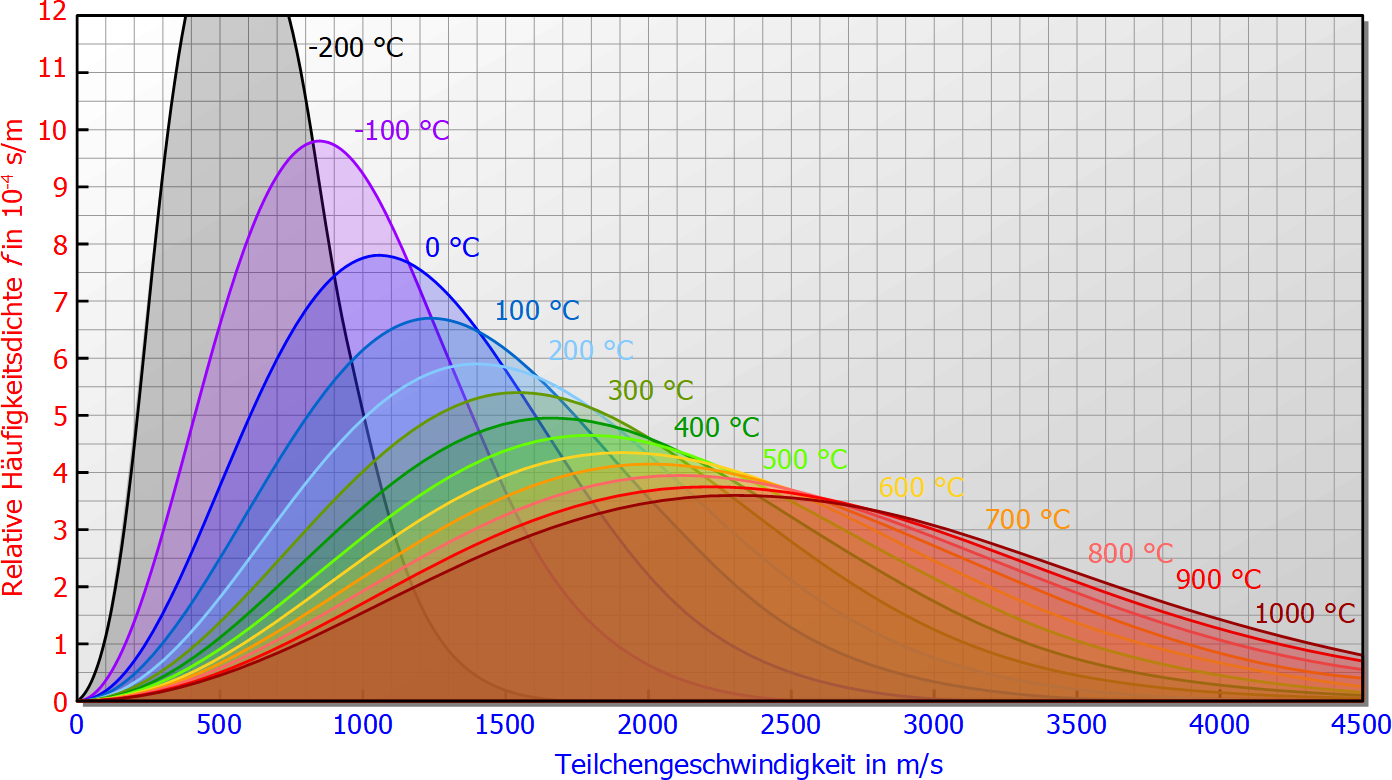
\includegraphics[width=0.75\textwidth]{img/boltzmann}
	\caption{Boltzmann-Verteilung}
\end{figure}
\FloatBarrier
%Ende

\newpage

\subsection{Allg. Beschreibung 1. HS Thermodynamik}
\begin{center}
	"`die innere Energie eines abgeschlossenen Systems bleibt konstant."'\\
	d$U=0$ bzw. $U=const.$
\end{center}

\textbf{\underline{Folgesätze, die sich daraus ergeben:}}
\begin{itemize}
	\item \textbf{Energieerhaltungssatz}:\\
	"`Energie kann weder erzeugt noch zerstört werden, sondern nur in eine andere Energieform umgewandelt werden."'
	\item Energie ist die Fähigkeit zum \textbf{Austausch von Arbeit und Wärme}
	\item innere Energie $ U $ und Enthalpie $ H $ beschreiben System als \textbf{Zustandsgrößen}
	\item In einem \textbf{Kreisprozess wird keine Energie gewonnen}, wenn bei Rückkehr auf einen beliebigen Weg vom Zustand 2 in den Ausgangszustand 1, die gleiche Summe von Wärme und Arbeit mit umgekehrten Vorzeichen ausgetauscht wird
\end{itemize}
\textbf{\underline{Arbeits- und Energietherme:}}
\begin{itemize}
	\item \textbf{Volumenarbeit} $W_V = F*s \rightarrow \text{d}W=p*A*\text{d}s=-p*\text{d}V $
	\begin{itemize}
		\item $U$ sinkt: Expansion
		\item $U$ steigt: Kompression
	\end{itemize}
	\textbf{Fall A:} Arbeit gegen $p_u,T=const.$
	\begin{flalign}
		&\text{d}W=-p*\text{d}V\\
		&\Delta W = W_2-W_1=\int_{V_1}^{V_2}-p_u\text{ d}V\\
		&\Delta W =-p_u\int_{V_1}^{V_2}\text{d}V=-p*(V_2-V_1)\\
 	\end{flalign}
 	\textbf{Fall B:} Arbeit gegen $T=const., p\neq const.$
 	\begin{flalign}
 	&\text{d}W=-p*\text{d}V\\
 	&\Delta W =\int_{V_1}^{V_2}-p\text{ d}V\\
 	&\Delta W =\int_{V_1}^{V_2}-\frac{n*R*T}{V}\text{ d}V\\
 	&\Delta W = -n*R*T* \int_{V_1}^{V_2}\frac{1}{V}\text{ d}V\\
 	&\Delta W = -n*R*T*\ln{\left(\frac{V_2}{V_1}\right)}
 	\end{flalign}
\end{itemize}

\newpage

\subsection{Totales Differential der inneren Energie U}
\begin{itemize}
	\item Abhängigkeiten von $U$ für ein gasförmiges System: $\text{ }U=f(p,T,V,n,...)$\\
	Innere Energie U (gasförmiges System) abhängig von Druck P, Volumen V, Temperatur T, Teilchenzahl n
	\item Beschreibung der Abhänigkeit von $U$ von den Größen p,T,V,... erfolgt als totales Differential\\
		\begin{flalign}
			\text{d}U &= \left(\frac{\partial U}{\partial T}\right)_{V,n}*\text{d}T+\left(\frac{\partial U}{\partial V}\right)_{T,n}*\text{d}V+\left(\frac{\partial U}{\partial n}\right)_{V,T}*\text{d}n
		\end{flalign}
		$\rightarrow$ für $n=const.$
		\begin{flalign}
		\text{d}U &= \left(\frac{\partial U}{\partial T}\right)_{V,n}*\text{d}T+\left(\frac{\partial U}{\partial V}\right)_{T,n}*\text{d}V
		\end{flalign}
		\begin{center}
			Wärmekapazität $c_V$ \hspace*{5mm} Binnendruck $\pi$\\
			bei $V=const.$ \hspace*{30mm}
		\end{center}
\end{itemize}

In jedem geschlossenem System ist jede infinitial kleine Änderung der Inneren Energie den jeweiligen Änderungen von Volumen und Temperatur proportional.\\
Proportionalitätsfaktoren sind dabei partielle Ableitungen nach den Zustandsvariablen $T,V \text{ und } n=const.$

\subsubsection{Temperaturabhängigkeit der inneren Energie $\mathbf{U}$}
\begin{flalign}
	\diff U &= \diff W +\diff Q\\
	Q_{12} &= (U_2-U_1)-W_{ges 1,2}\\
	q_{1,2} &= (u_2-u_1)-w_{ges 1,2}
\end{flalign}
Nur Volumenarbeit, vollständig reversibler Prozess\\

\begin{table}[h!]
	\centering
	\begin{tabulary}{1.15\textwidth}{C|C|C}
		System mit $p=const.$ u. $p\neq f(V)$ & System mit $p\neq const.$ & System mit konst. Volumen $\diff W_{Vol}=0$ \\  
		$q_{12}=(u_2-u_1)-p*(v_2-v_1)$& $q_{12}=(u_2-u_1)-n*R*T*\ln\left(\frac{v_2}{v_1}\right)$ & $q_{12}=(u_2-u_1)$
	\end{tabulary} 
\end{table}
\FloatBarrier

\newpage

\subsubsection{Wärmekapazität $\mathbf{c_V}$ bei konstantem Volumen}
\begin{flalign}
	\diff U =\left(\frac{\partial U}{\partial T}\right)_{V,n}*\diff T
\end{flalign}
\vspace*{-5mm}\\
\hspace*{70mm} $\hookrightarrow c_V$\\
\begin{itemize}
	\item $c_V$ gibt an wie stark sich die innere Energie des Systems mit der Temperatur $(v=const.)$|adiabat
	\item $c_V=$"'groß"': \\
	hohe Wärmekapazität, stärkere Änderung von $U$, Teilchen können "`viel"' Energie aufnehmen 
	\begin{itemize}
		\item frei beweglich
		\item  viele Teilchen
		\item Rotation, Translation, Vibration
		\item wenig Doppelbindung
	\end{itemize}
	\item Wärmekapazität ist selbst wieder eine temperaturabhängige Größe\\
	Generell gilt:
	\begin{itemize}
		\item für $T\rightarrow \SI{0}{\kelvin}$ mit $c_V \rightarrow 0$
		\item für Phasenwechsel mit $c_V\rightarrow \infty$
	\end{itemize}
\end{itemize}

\subsubsection{Volumenabhängigkeit der inneren Energie $\mathbf{U}$}
\textbf{Der Binnendruck $\mathbf{\pi}$}
\begin{flalign}
	\diff U &= \left(\frac{\partial U}{\partial T}\right)_{V,n}*\diff T+\left(\frac{\partial U}{\partial V}\right)_{T,n}*\diff V
\end{flalign}
für $n=const.$
\begin{flalign}
	\diff U &= c_v+\diff T + \pi *\diff V
\end{flalign}
\vspace*{-10mm}\\
\hspace*{85mm} $\uparrow$ Binnendruck

Der Binnendruck $\pi$ ist eine Maß für die Änderung der inneren Energie eines Stoffes, wenn sich Volumen bei $T=const.$ ändert

\begin{table}[h!]
	\centering
	\begin{tabulary}{1.15\textwidth}{C|C}
		\textbf{Ideale Gase} & \textbf{Reale Gase}\\
		\hline
		$\pi =0$ 	& $\pi \uparrow$ - Abstoßung der Teilchen\\
		& $\pi \downarrow$ - Anziehung der Teilchen\\
		keine WW der Teilchen & WW zwischen den Teilchen
	\end{tabulary} 
\end{table}
\FloatBarrier

\newpage

\section{Modellsystem "`Ideales Gas"' und Verhalten realer Gase}
\subsection{Annahmen zum idealen Gas}
\begin{itemize}
	\item Energie nur in Form kinetischer Energie\\
	$\rightarrow$ potentielle Energie wird aufgrund WW mit Atomen/Molekülen vernachlässigt
	\item Stöße zwischen Teilchen vollständig elastisch\\
	$\rightarrow$ keine E-Umwandlung durch Verformung,...
	\item kein Eigenvolumen der Teilchen
	\item Teilchen sind in zufälliger Bewegung zueinander (kontinuierlich)\\
	$\rightarrow$ Energie verteilt sich auf Energieniveaus\\
	$\rightarrow$ Verteilung der Teilchengeschwindigkeit 
	\item Größe der Teilchen vernachlässigbar, da $<<<$ mittlere, freie Weglänge \\
	("`Weg vor Stoß"')
\end{itemize}


\subsection{Verhalten realer Gase}

\begin{itemize}
	\item WW der Teilchen
	\item Eigenvolumen
	\item inelastische Stöße
	\item statistisch nicht mehr zufällige Bewegung
\end{itemize}

\textbf{KONSEQUENZ:}\\
Die Zustandsgrößen $p$ und $V$ zeigen in der/ihrer Berechnung Abweichungen, wenn sie nicht mit einem entsprechenden korrigierten Gasgesetz bestimmt bzw. berechnet werden.

\begin{center}
	\textbf{Übergangslösung:}
	\begin{itemize}
		\centering
		\item bei Experiment hohe Temperaturen und niedrige Drücke
		\item Nutzung des ideales gases zum Überblick
	\end{itemize}
\end{center}

\newpage

\textbf{LÖSUNGSMÖGLICHKEITEN:}
\begin{itemize}
	\item \textbf{Einsatz von Korrekturfaktoren}
	\begin{itemize}
		\item Kompressibilität $z$
		\item Fugazitäten- und Fugazitätskoeffizienten $f_{\text{i}}$ und $\Phi_{\text{i}}$
		\item Aktivität- und Aktivitätskoeffizienten $a_{\text{i}}$ und  $\gamma_{\text{i}}$\\
			$a_{\text{i}}=\gamma_{\text{i}}*c_{\text{i}}$ mit $\gamma_{\text{i}}=1,0$ als 100\% ideal
	\end{itemize}
	
	\item \textbf{Erweiterung des idealen Gasgesetzes}
	\renewcommand{\arraystretch}{1.2}
	\begin{table}[h!]
		\centering
		\begin{tabulary}{\textwidth}{C|C}
			\textit{Erweiterung durch die Einführung von Zusatzgliedern} & \textit{Einführung von Korrekturtermen in das ideale Gasgesetz} \\
			\hline
			&\\
			Reihenentwicklung & Korrekturtherme\\
			"`Virialgleichungen"'& Van-der-Waals GL, Berthelot GL, Redlich-Kwong GL, Peng-Robinson GL
		\end{tabulary} 
	\end{table}
	\FloatBarrier
\end{itemize}








\subsection{Zustandsgleichung und Gasgesetze}
\subsubsection{Charakterisierung der Gasphase am Beispiel von Wasser-Dampf-Gemischen}
System A = \\
Mischung aus flüssiger Phase (F,$'$) und gasförmiger Phase (Dampf D, $''$)
\begin{flalign}
	V_A &= m_D*V''+m_F*V'\\
	V_{m_A} &= \frac{V_A}{n} \quad V_A = \frac{v_A}{m_A}\\
	\chi_{\text{i}} &= \frac{n_{\text{i}}}{n_{\text{ges}}} = \frac{m_{\text{i}}}{m_{\text{ges}}}\\
	v_A &= \chi_D *v''+\chi_F*v'\\
		&= \chi_D *v''+(1-\chi_D)*v'\\
		&= \chi_D *v''+v'-\chi_D*v'\\
		&= v''+\chi_D*(v''-v')\\
	\chi_D &=\frac{v_A-v'}{v''-v'}
\end{flalign}

\begin{itemize}
	\item Eigenschaften der D-F-mischung sind abhängig von den Massen- bzw. Molenbrüchen der Phasen
	\item Jedes Zweiphasengebiet kann jeden Punkt genau durch Temperatur und Druck bestimmen \\
	$\rightarrow$ Freiheitsgrad = 1 $\rightarrow F=K-P+2$
	\item Dampf-Tafeln für verschiedene Stoffsysteme mit spezifischen Zustandsgrößen $v,h,s$
\end{itemize}

\subsubsection{Analoge Betrachtung für ander thermodynamische Größen}
\textbf{Enthalpie:}\\
\begin{flalign}
	H_A 	&= m_D * H'' +m_F*H'\\
	\chi_D 	&= \frac{h_A-h'}{h''-h'}\\
	h_A		&= \chi_D*(h''-h')+h'
\end{flalign}
\textbf{Entropie:}\\
\begin{flalign}
S_A 	&= m_D * S'' +m_F*S'\\
\chi_D 	&= \frac{s_A-s'}{s''-s'}\\
s_A		&= \chi_D*(s''-s')+s'
\end{flalign}


\subsection{Kinetische Gastheorie}

ABBILDUNG \\

\textbf{Reduzierte Masse $\mathbf{\mu}$}
\begin{flalign}
	\mu 		&= m_{Red} \quad \quad \quad \quad \quad \quad \text{(einatomig)}\\
	\mu &= m_{Red} = \frac{m_1*m_2}{m_1+m_2} \text{ (zweiatomig)}
\end{flalign}

\subsubsection{Impuls und Impulsänderung}

\begin{enumerate}
	\item 	\begin{flalign}
				\Delta p_x 	&= \mu*V_X-\mu *(-V_x)\\
							&= 2 \mu * V_x
			\end{flalign}
	\item Für zwei Treffer auf eine Wand muss ein Teilchen 2x die Strecke $l$ zurücklegen
	\begin{flalign}
				\Delta t= \frac{2*t}{V_x}
	\end{flalign}
	\item Für die ausgeübte Kraft (=Druck) an der Wand ergibt sich:
	\begin{flalign}
		F &= \frac{\Delta p_x}{\Delta t} = \frac{\mu*V_x^2}{l}\\
		p_{{\tiny Druck}} &=\frac{F}{A} = \frac{\mu*V_x^2}{l*A} = \frac{\mu*V_x^2}{V}
	\end{flalign}
	\item Berücksichtigung der Teilchenzahl $N$ (ausschließlich translatorische Freiheitsgrade x-Richtung)
	\begin{flalign}
		\bar{v}^2 	&= v_x^2+v_y^2+v_z^2\\
		p*V 		&= \frac{1}{3}*N*\mu*\bar{v}^2	 
	\end{flalign}
	Für 1 mol Teilchen ergibt sich:
	\begin{flalign}
		N 	&= n*N_A \\
		n 	&= \frac{m}{M}=\frac{\mu}{M}\\
		p*V &= n*M_{ges}*\bar{v}^2
	\end{flalign}
	\item Wenn die neu gefundene Gleichung als Zustandsgleichung für das ideale Gas gelten soll, können wir nachfolgend auch den Ausdruck $n*R*T$ mit in die Gleichung integrieren
	\begin{flalign}
		\frac{1}{3}*N*\mu*\bar{v}^2 &= n*R*T\\
		\frac{1}{3}*n*M_{ges}*\bar{v}^2 &= n*R*T\\
	\end{flalign}
	\begin{flalign}
		k_B &= \SI{1,38e-23}{\joule \per \kelvin}\\
		R 	&= \SI{8,314}{\joule\per\kelvin\per\mole}\\
		N_A &= \SI{6,02e23}{\per\mole}
	\end{flalign}
	$\rightarrow$ mit $R=k_B*N_A$ \\
	\begin{flalign}
		\bar{v} 	&= \sqrt{\frac{3*R*T}{N*\mu}}\\
					&= \sqrt{\frac{3*R*T}{M}}\\
					&= \underline{\underline{\sqrt{\frac{3*k_B*T}{\mu}}}}
	\end{flalign}
	\item \textbf{Schlussfolgerung:}
	\begin{flalign}
		\bar{v}^2 \sim T \text{ und } \bar{v}^2 \sim \frac{1}{\mu} \text{ bzw. } \frac{1}{M}\\
		p*V = N *k_B*T
	\end{flalign}
\end{enumerate}

\subsubsection{Boltzmann Verteilung}

ABBILDUNG\\

=Beschreibt Einfluss von $T$ auf Geschwindigkeitsverteilung der Teilen, sowie der Molmasse $M$ bzw. reduzierten Masse $\mu$

\subsubsection{Mittlere quadratische Geschwindigkeit $\mathbf{\bar{v}}$}
\begin{flalign}
	\bar{v}^2 	&= \frac{3*R*T}{M}\\
	\bar{v}		&= \sqrt{\frac{3*R*T}{M}}
\end{flalign}
\underline{Bsp.:} $CO_2$ mit $\bar{v}= \SI{411}{\meter \per \second}$

\subsubsection{Mittlere Geschwindigkeit $\mathbf{c}$}
\begin{itemize}
	\item aus Maxwell Gleichung
	\item jede Geschwindigkeit wird multipliziert mit Teilchenzahl, die diese Geschwindigkeit besitzen
	\item Aufsummation aller Produkte und Mittelung
\end{itemize}
\begin{flalign}
	c 		&= \int_{0}^{\infty} s*f(s)*\diff s\\
	f(s) 	&= 4*\pi*\left(\frac{M}{2*\pi*T*R}\right)^{\frac{3}{2}}*s^2*e^{-\frac{M*s^2}{2*R*T}}\\
	c		&= 4*\pi*\left(\frac{M}{2*\pi*T*R}\right)^{\frac{2}{3}}*\frac{1}{2}*\left(\frac{2*R*T}{M}\right)^2\\
	c		&= \underline{\underline{\left(\frac{8*R*T}{\pi*M}\right)^{\frac{1}{2}}}}
\end{flalign}


\section{Kenngrößen zur Beschreibung realer Gassysteme}
\subsubsection{Kompressibilitätsfaktor $\boldsymbol{Z}$}
\begin{flalign}
	Z	&= \frac{V_{\text{Real}}}{V_{\text{Ideal}}}=\frac{V_{\text{m}}}{V_{\text{m, Ideal}}}=\frac{p*V_{\text{Real}}}{n*R*T}
\end{flalign}
\begin{itemize}
	\item Einführung eines Idealitätsfaktors (Abhängig von Druck und Temperatur)
	\item $Z=1$: ideales Gas bzw. Verhalten von idealen Gasen
	\item $Z>1$: Abstoßungskräfte, Gas schwerer als ideales Gas komprimierbar
	\item $Z<1$: Anziehungskräfte, Gas leichter als ideales Gas komprimierbar
\end{itemize}

ABBILDUNG

\subsubsection{\textsc{Boyle} Temperatur}
= Temperatur bei der die Eigenschaften des realen Gases mit den eines idealen Gases für $p \rightarrow 0$ übereinstimmen
\begin{itemize}
	\item $T>T_B$: Isothermen haben nur ansteigenden Charakter
	\item $T<T_B$: Isothermen zeigen ein Minimum auf
\end{itemize}
$\rightarrow$ anziehende WW-Kräfte zeigen bei tiefen Temperaturen einen stärkeren Effekt\\
$\rightarrow$ eine unbegrenzte Annäherung ist aber nicht möglich, für hohe Drücke dominieren Abstoßungskräfte\\ \\
\underline{Bsp.:} \hspace{7mm} $T_B(\ce{CO2})=500\si{\celsius}$

\subsection{Die Virialgleichung}
\underline{Ansatz:}\\
Erweiterung der Gleichung des idealen Gases durch die Einführung von zusätzlichen Gliedern\\
$\rightarrow$ Reihenentwicklung nach $p$ oder $V_m$
\begin{itemize}
	\item für techn. Anwendung Abbruch der Reihenentwicklung nach dem 2. oder 3. Glied
	\item kann nur dampfförmige Zustände beschreiben
	\item nutzbar bis $\approx \frac{1}{3}$ der kritischen Dichte (vom Druck $p$)
	\item Virialkoeffizienten $B,D,...$ sind abhängig von der Temperatur und der Zusammensetzung (Konzentrationen) des Stoffsystems
\end{itemize}
\begin{flalign}
	p*V_m &= R*T\\
	p*V_m &= R*T+B(T)*p+C(T)*p^2+D(T)*p^3+...\\
	p*V_m &= R*T*\left(1+\frac{B'}{V_m}+\frac{C'}{V_m}+...\right)
\end{flalign}
\newpage
\subsection{Die \textsc{Van-der-Waals}-Gleichung}
\textit{Einführung zusätzlicher Terme in das ideale Gasgesetz} \\

ABBILDUNG\\

$\rightarrow$ \textsc{Van-der-Waals}-Koeffizienten $a$ und $b$\\
= Parameter stoffspezifisch und für übliche Stoffsysteme tabelliert

\subsubsection{Der \textsc{Van-der-Waals}-Koeffizient $\boldsymbol{a \left[\si{\pascal \raiseto{6} \meter \per \raiseto{2} \mol}\right]}$ - Kohäsionsdruck}
Über diesen Term werde die WW zwischen den Teilchen erfasst:
\begin{flalign}
	p_{\text{{\tiny ideal}}} &= p_{\text{{\tiny real}}} + p_{\text{{\tiny Kohäsion}}}
\end{flalign}
\textit{Ansatz}:
\begin{flalign}
	p_{\text{{\tiny Kohäsion}}} &= \frac{a}{(V_m)^2}
\end{flalign}
\textit{Hintergrund}:\\
Druck $p$ = Stoßhäufigkeit und Kraft der Stöße
\begin{flalign}
	p &\sim \frac{n}{V}\\
	V_m &\sim \frac{V}{n}
\end{flalign}
Aus dem \textsc{Coulomb}'schen Gesetz folgt, dass die WW = Stärke in quadratischer Abhängigkeit zum Abstand steht

\subsubsection{Der Van-der-Waals-Koeffizient $\boldsymbol{b}\left[\si{\raiseto{3}\centi\meter\per \mole}\right]$ - Kovolumen}
\begin{flalign}
	V_{\text{m, ideal}} &= V_m-V_{\text{m, korr}}
\end{flalign}

\textit{Ansatz:}
\begin{flalign}
	V_{\text{m, korr}} &= n*b
\end{flalign}

\textit{Hintergrund:}
\begin{flalign}
V_{\text{m, korr}} &= n*b
\end{flalign}
\begin{itemize}
	\item Moleküle bzw. Gasteilchen können sich nicht im gesamten Volumen bewegen, sondern nur im Volumen \\
	$\Rightarrow V-n*b$
	\item der kleinstmögliche Abstand zwischen zwei Kugeln beträgt \\
	$\Rightarrow$ $2*r$ (r-Radius)\\ \\
	\newpage
	$\rightarrow$ daraus folgt für eine Bewegung zwischen 2 Kugeln ein Volumen von $8*V_{\text{Molekül}}$ nicht zugänglich ist (3D: $2^3=8$)
	\begin{itemize}
		\item 4x $V_{\text{Molekül}}$ ist nicht zugänglich
		\item bzw. $b\sim 4*V_{\text{Molekül}}*N_A$
	\end{itemize}
	$\rightarrow$ über diesen Term wird das Eigenvolumen der Teilchen berücksichtigt
	\item Für bzw. mit beiden Termen zusammen erweitert bzw. modifiziert sich die allgemeine Gasgleichung zu:
	\begin{flalign}
		p 	&= \frac{n*R*T}{V-n*b}-a*\frac{n^2}{V^2} \\
			&= \frac{R*T}{V_m-b}-\frac{a}{V^2_m}
	\end{flalign}
\end{itemize}

\subsubsection{Anwendung:}
Die \textsc{Van-der-Waals}-Gleichung beschreibt das Verhalten realer Gase einschließlich ihres kritischen Verhaltens und im 2-Phasen-Gebiet (flüssig/gasförmig)\\ \\

ABBILDUNG\\ \\

\subsubsection{Zusammenhang der \textsc{Van-der-Waals}-Gleichung mit den kritischen Größen}
\begin{itemize}
	\item Für Temperaturen $T>T_{Kr}$ zeigen die Isothermen einen stetigen Anstieg zu höheren Drücken und kleinen Volumina
	\item Für Temperaturen  $T<T_{Kr}$ zeigen die Isothermen jeweils ein Minimum und ein Maxima
	\item Für Temperaturen $T\rightarrow T_{Kr}$ nähern sich die Extrema Minimum und Maximum soweit zueinander an, dass sie in Form eines Wendepunkts zusammenfallen. Am kritischen Punkt hat die Isotherme damit einen Anstieg von 0
\end{itemize}

\newpage

\subsubsection{Bestimmung der kritischen Zustandsgrößen}
\begin{flalign}
	p								&= \frac{R*T}{V_m-b}-\frac{a}{(V_m)^2}\\
	\frac{\diff p}{\diff V_m}		&= -\frac{R*T}{(V_m-b)^2}+\frac{2*a}{(V_m)^3}\\
	\frac{\diff^2 p}{\diff (V_m)^2}	&= +\frac{R*T}{(V_m-b)^3}+\frac{6*a}{(V_m)^4}
\end{flalign}
\begin{flalign}
		V_{m_{krit}} 	&=3*b \\
		T_{Kr}			&=\frac{8a}{27*R*b} \\
		p_{krit} 		&=\frac{a}{27*b^2}\\[2mm]
		Z_{krit}		&=\frac{V_{real}}{V_{ideal}} = \frac{p_{krit}*V_{m_{krit} }}{R*T_{Krit}}
\end{flalign}

\subsubsection{Reduzierte Zustandsgrößen \textsc{Van-der-Waals}-Gleichung}
$\rightarrow$ die kritischen Zustandsgrößen $p_{krit}, T_{krit}, V_{krit}$ sind für die einzelnen Gase charakteristischer bzw. stoffspezifisch, aber sie sind für alle Gase vorhanden bzw. existent \\
Nutzung dieser fundamental für alle Gase vorhandenen und geltenden Größen, um darauf eine relative Vergleichsskala aufzubauen \\ \\
\textit{\underline{Wie:}}\\
Normierung der $p,T,V$-Werte auf die jeweilige kritische Größe unter Einführung sogenannter reduzierter Größen $p_R,V_R,T_R$
\begin{flalign}
	T_R		&= \frac{T}{T_{Krit}}\\
	p_R		&= \frac{p}{p_{Krit}}\\
	V_R		&= \frac{V}{V_{Krit}}\\[2mm]
	V_{m_R}		&= \frac{V_m}{V_{m_{Krit}}}
\end{flalign}

\newpage

\subsubsection{Grenzen und Gültigkeit der \textsc{Van-der-Waals}-Gleichung}
\begin{itemize}
	\item \textsc{Van-der-Waals}-Gleichung\\
	= Beschreibung des Verlaufs und Zusammenhang der Zustandsgrößen $p,V,T$ der Gas- und Flüssigphase qualitativ richtig und hingehend genau\\ \\
	$\rightarrow$ Für besonders exakte Analysen sowie im Bereich sehr hoher Drücke gibt es heute jedoch genauere Gleichungen (\textsc{Redlich-Kwong},...)
	\item  Für hohe Temperaturen und große molare Volumen ist die \textsc{Van-der-Waals}-Gleichung gut anwendbar und geht im Grenzfall aufgrund:\\
	\begin{flalign}
		V_m >> b
	\end{flalign}
	und der Dominanz des ersten Gleichungssystems
	\begin{flalign}
	\frac{R*T}{V_m-b} >> \frac{a}{(V_m)^2}
	\end{flalign}
	in das ideale Gasgesetz über.
	\begin{flalign}
		p 		&= \frac{R*T}{V_m-\cancel{b}}-\cancel{\frac{a}{(V_m)^2}}\\
		p*V_m	&= R*T\\
		p*V		&= n*R*T
	\end{flalign}
\end{itemize}

\subsection{Die \textsc{Redlich-Kwong}-Gleichung}
\subsubsection{Allgemeine Infos zur \textsc{Redlich-Kwong}-Gleichung:}
\begin{itemize}
	\item empirische Erweiterung der  \textsc{Van-der-Waals}-Gleichung von  \textsc{Redlich} und \textsc{Kwong} im Jahr 1949
	\item für:
		\begin{itemize}
			\item $T>T_{Krit} \rightarrow 1$ reelle Lösung der Gleichung 
			\item $T<T_{Krit} \rightarrow 3$ reelle Lösungen der Gleichung 
		\end{itemize}
	$\rightarrow$ gleicher Schleifenförmiger Verlauf der Funktion\\
	$\rightarrow$ Indikator für 2-Phasen-Gebiet
	\item Auch aus der  \textsc{Redlich-Kwong}-Gleichung können die kritischen Größen berechnet bzw. umgekehrt die Parameter $a$ und $b$ aus diesen bestimmt werden
\end{itemize}
\subsubsection{Extensive Form der \textsc{Redlich-Kwong}-Gleichung:}
\begin{flalign}
	\left(p+\frac{a*n^2}{V*(V+n*b)*T^{0,5}}\right)*(V-n*b)&=n*R*T
\end{flalign}
\subsubsection{Intensive Form der \textsc{Redlich-Kwong}-Gleichung:}
\begin{flalign}
\left(p+\frac{a}{V_m*(V_m+b)*T^{0,5}}\right)*(V_m-b)&=R*T
\end{flalign}
\begin{flalign}
b	&= (2^{\frac{1}{3}}-1)*V_{krit}\\
a	&= \frac{1}{3*(2^{\frac{1}{3}}-1)}*R*T^{\frac{2}{3}}_{krit}*V_{krit}
\end{flalign}

\subsection{Die \textsc{Peng-Robinson}-Gleichung}
\subsubsection{Allgemeine Infos zur \textsc{Peng-Robinson}-Gleichung:}
\begin{itemize}
	\item Erweiterung der \textsc{Redlich-Kwong}-Gleichung durch \textsc{Peng} und \textsc{Robinson} im Jahr 1976
	\item Wiederum können auch aus der \textsc{Peng-Robinson}-Gleichung die kritischen Größen berechnet werden
	\begin{flalign}
		p	&= \frac{R*T}{V_m-b} - \frac{a(T)}{(V_m)^2+2b*V_m-b^2}\\[2mm]
			&= \frac{R*T}{V_m-b} - \frac{a(T)}{(V_m)*(V_m+b)+b*(V_m-b)}
	\end{flalign}
	\begin{flalign}
		b	&= 0,0778*\frac{R*T_{\text{{\tiny Krit}}}}{p_{\text{{\tiny Krit}}}}\\[2mm]
		a	&= 0,457*\frac{R^2*T^2_{\text{{\tiny Krit}}}}{p_{\text{{\tiny Krit}}}}
	\end{flalign}
\end{itemize}

\section{Die Enthalpie $\boldsymbol{H}$}
\subsection{Die Enthalpie in techn. Prozesse}

ABBILDUNG \\
\begin{flalign}
	  p_1 			&= p_2 = const.\\
	  W_{mech_{12}}	&= W_{mech_{Rev_{12}}}+W_{mech_{diss_{12}}}\\
	  W_{ges_{12}}	&= W_{vol_{12}}+W_{mech_{12}}\\
	  \diff U 		&= \diff W + \diff Q
\end{flalign}
$\rightarrow$\textit{adiabatisches System,} $\diff Q=0$
\begin{flalign}
\diff U 	&= \diff W_{ges} = \diff W_{vol_{12}}+\diff W_{mech_{12}}
\end{flalign}
\begin{flalign}
\diff W_{vol}	&= -p*\diff V
\end{flalign}
\textit{bei } $p=const.$ \textit{mit} $\Delta W_{vol}=-p*\Delta V$\\[1.mm]
\textit{bei } $p=\frac{n*R*T}{V}$ \textit{mit} $\Delta W_{vol}=-\int_{V_1}^{V_2}\frac{n*R*T}{V}*\diff V=-n*R*T*\ln\left(\frac{V_2}{V_1}\right)$\\
\newpage
$\rightarrow$\textit{Isobares System, }$p=const.$
\begin{flalign}
	\Delta W_{ges}	&= \Delta W_{mech_{12}}+\left[(p*V_1)-(p*V_2)\right]\\
					&= \Delta U \\
					&= U_2-U_1
\end{flalign}
$\rightarrow$\textit{Umstellen nach }$\Delta W_{mech_{12}}$
\begin{flalign}
\Delta W_{mech_{12}}	&= (U_2+p*V_2)-(U_1+p*V_1)\\
						& \hspace{1.5cm} H_2 \hspace{2cm} H_1
\end{flalign}
$\rightarrow$\textit{Einführung der neuen Zustandsgröße Enthalpie $H$}\\ \\
Die Enthalpie $H$ berücksichtigt, die bei $p=const.$ zu leistende Volumenverschiebearbeit. Sie setzt sich aus der inneren Energie $U$ und der Verschiebearbeit $\Delta W_{mech_{12}}$ zusammen.
\begin{flalign}
	H	&= U+p*V
\end{flalign}

\subsection{Die Enthalpie in der Chemie}
Der Wärmeaustausch hat bei phys.-chem. Prozessen und bei chem. Reaktionen oft die größte Bedeutung, z.B. therm. Aktivierung von chem. Reaktionen (\textsc{Arrhenius} Aktivierungsenergie), räumliche Umstrukturierung (cis-/trans-Isomerien) und die WW zwischen den Teilchen/Phasenübergänge (Schmelzen, Sieden, Mischungsbildung)\\
$\rightarrow$\textit{Für isochore Prozesse }$\diff V =0$, \textit{gilt} $\diff U=\diff Q$ \textit{(selten der Fall)}\\
$\rightarrow$ \textit{chem.-physk. Prozesse und chem. Reaktionen verlaufen jedoch oft \underline{isobar}, statt \\
\hspace*{0.5cm}isochor}\\
\hspace*{2cm} $\rightarrow$ Reaktionen und Prozesse in offenen Systemen oder bei konstanter\\
\hspace*{2.6cm} Pumpleistung bzw. Druckregelung\\
$\rightarrow$\textit{\textbf{Folge:}}\\
\hspace*{0.5cm}Neben dem Wärmeaustausch wird gleichzeitig auch Volumenarbeit verrichtet
\begin{flalign}
	\diff U 				&= \diff W + \diff Q\\
	\diff W= \diff W_{vol} 	&=-p*\diff V\\
	\Delta W_{vol}			&= -p*\Delta V \\
							&=-p*(V_2-V_1)
\end{flalign}
\textit{Umstellen nach} $\diff Q$ \textit{bzw.} $\Delta Q$
\begin{flalign}
	\Delta Q_{12} 	&= \Delta U_{12} - (-p*\Delta V_{12})\\
					&= U_2-U_1-[-p*(V_2-V_1)]\\
					&= (U_2-p*V_2)-(U_1-p*V_1)\\
					& \hspace{1.5cm} H_2 \hspace{2cm} H_1
\end{flalign}
\textit{für} $p =const.$
\begin{flalign}
 \Delta Q &= H_2-H_1 = \Delta H_{12}
\end{flalign}

\subsection{Die Enthalpie $\boldsymbol{H}$ eines Systems}
\begin{flalign}
	H &= U + p*V\\
	\diff H &= \diff U + p*\diff V + V*\diff p
\end{flalign}
$\rightarrow \diff U = \diff W + \diff Q$ \textit{mit} $\diff W =\diff W_{vol}$\\
$\rightarrow \diff U = -p*\diff V+\diff Q$
\begin{flalign}
	\diff H &= -p*\diff V+\diff Q +p*\diff V + V*\diff p\\
			&= V*\diff p+\diff Q
\end{flalign}
$\rightarrow$ \textit{Kombination mit dem idealen Gasgesetz }$p*V=n*R*T$
\begin{flalign}
	H	&= U+n*R*T\\
\end{flalign}
$\rightarrow$ \textit{spezifische Enthalpie}
\begin{flalign}
	H_{sp}	&= h_{sp} = \frac{H}{m}\\[1mm]
	H_m		&= h_m =\frac{H}{n}
\end{flalign}
\subsubsection{Zusammenfassung}
\begin{itemize}
	\item die Enthalpie H ist eine zusammengesetzte Größe aus innerer Energie und einer Volumen(-verschiebe)arbeit
	\item Enthalpie ist eine Zustandsgröße
	\item $H$ trägt die Einheit einer Energie $\left[\si{\joule}\right]$
	\item die Enthalpie wird primär zur Beschreibung thermodyn. Prozesse und chem. Reaktionen in der Chemie genutzt
\end{itemize}
$\boldsymbol{\rightarrow}$ {\large\textbf{ Es gilt:}} \hspace{10mm}$\boldsymbol{U<H}$\\
Berücksichtigung der Volumenarbeit bei chem-phys. Prozessen und chem. Reaktionen
\newpage
\subsection{Die Enthalpie phys. Prozesse und chem. Reaktionen}
\begin{itemize}
	\item grundsätzlich ist die Enthalpie von den Zustandsgrößen $p,V,T$ und $n$ abhängig
	\begin{flalign}
		H	&= f(n,p,T,V,...)
	\end{flalign}
	\item Erfassung als Funktionsgleichung über das totale Differential
	\begin{flalign}
		\diff H &= \left(\frac{\partial H}{\partial p}\right)_{n,T}*\diff p+\left(\frac{\partial H}{\partial T}\right)_{n,p}*\diff T+\left(\frac{\partial H}{\partial n}\right)_{p,T}*\diff n
	\end{flalign}
	$\rightarrow$\textit{für $n=const.$}
		\begin{flalign}
	\diff H &= \hspace{0.7cm}\left(\frac{\partial H}{\partial p}\right)_{n,T}*\diff p+\hspace{1cm}\left(\frac{\partial H}{\partial T}\right)_{n,p}*\diff T
	\end{flalign}
	\hspace{4cm} Isothermer \hspace{3cm}Wärmekapazität $c_p$\\
	\hspace*{3cm}\textsc{Joule-Thomson}-Koeffizient\hspace{1.5cm}bei $p=const.$\\
	\hspace*{5cm}$\mu_T$\\
	$\rightarrow \mu_T=-c_p*\mu$ \\ \\
	$\boldsymbol{\mu}$ = isenthalpischer \textsc{Joule-Thomson}-Koeffizient der dem Verhältnis zwischen Temperatur- und Druckänderung bei der Expansion \linebreak eines Gases unter $H=const.$ entspricht
	\item In einem geschlossenen System ist jede infinitesimale Änderung der \linebreak
	Enthalpie $H$ den jeweiligen Änderungen von Druck und Temperatur proportional ($n=const.$)\\ \\
	Die Proportionalitätsfaktoren sind dabei die partiellen Ableitungen nach $T$ bzw. $p$ und entsprechen der Wärmekapazität $c_p$ bei $p=const.$ und dem isothermen \textsc{Joule-Thomson}-Koeffizient $\mu_T$
\end{itemize}
\newpage
\subsubsection{Wärmekapazität bei $\boldsymbol{p=const.}$}
\begin{itemize}
	\item die Wärmekapazität $c_p$ bei $p=const.$ gibt an, wie stark sich die Enthalpie eines Systems mit der Temperatur bei konstantem Druck ändert.\linebreak
	Da für isobare Prozesse gilt: $\frac{V}{T}=const.$ ist dieser Prozess mit einer Volumenzu- oder -abnahme verbunden.
	\item $c_p$ kann als molare bzw. auch spezifische Größe oder als absolute Größe $c_p$ angeben werden.
	\begin{flalign}
		c_p	&= \frac{C_p}{n}
	\end{flalign}
	\underline{Bsp.:} molare Wärmekapazitäten $c_p$
	\begin{itemize}
		\item \ce{Ar}: $\SI{20.76}{\joule \per \kelvin \per\mole}$
		\item \ce{H2O}: $\SI{75.79}{\joule \per \kelvin \per\mole}$
		\item \ce{H2O} $(liquid, 298K)$: $\SI{4.18}{\kilo\joule \per \kelvin \per\kg}$
	\end{itemize}
	\item \underline{vollständige differentielle Abhängigkeit von $H$:}\\ \\
	$\rightarrow$\textit{für $n=const.$ und $p=const.$}
	\begin{flalign}
		\diff H &= \left(\frac{\partial H}{\partial T}\right)_{p,n}*\diff T=c_p*\diff T\\[1mm]
		H		&= U+p*V\\
		\diff H &= V*\diff p+\diff Q
	\end{flalign}
	$\rightarrow$\textit{für $n=const.$ und $p=const.$ gilt: $\diff H=\diff Q$}
	\begin{flalign}
		\diff Q &= c_p*\diff T
	\end{flalign}
	\item \underline{Abhängigkeiten von $c_p$:}
	\begin{itemize}
		\item $c_p$ ist temperaturabhängig:
			\begin{itemize}
				\item $c_p \rightarrow 0$ für $T \rightarrow \SI{0}{\kelvin}$
				\item $c_p \rightarrow \infty$ für Phasenwechsel
			\end{itemize}
		\item $c_p$ ist umso größer, je mehr "`Energie"' das Vielteilchensystem aufnehmen kann.\\
		Dies ist unter anderem abhängig von der ANzahl an besetzbaren energetischen Zuständen auf Ehrenbruderbasis von Translation, Rotation und Vibration\\
		$\rightarrow c_p$ = stoffspezifisch und abhängig von der Phase bzw. Erscheinungsform des Stoffes $(s,l,g)$ 
	\end{itemize}
	$\Rightarrow$ \underline{Besonderheiten:}
	\begin{itemize}
		\item $c_p>c_v$, da zusätzlich Arbeit zur isobaren Volumenvergrößerung aufgebracht werden muss
		\item $c_p$ und $c_v$ stehen in einem Zusammenhang zum Adiabatenkoeffizient $\kappa$ bzw. $\beta$
	\end{itemize}
	\newpage
	\item \underline{Die Temperaturabhängigkeit von $c_p$}\\ \\
	$\rightarrow$\textit{für $n,p =const.$}
	\begin{flalign}
		\diff H 	&= \left(\frac{\partial H}{\partial T}\right)_{n,p}*\diff T\\
		\diff H		&= c_p*\diff T
	\end{flalign}
	\begin{itemize}
		\item \textbf{Fall 1:}\\
		$c_p$ soll $\neq f(T)$ sein, möglich bei kleinen $\Delta T$
		\begin{flalign}
			\Delta H 	&= \int_{T_1}^{T_2}c_p*\diff T\\
						&= c_p*\int_{T_1}^{T_2}*\diff T\\
						&= c_p*(T_2-T_1)
		\end{flalign}
		\item \textbf{Fall 2:}
		\begin{itemize}
			\item \textit{\underline{Ansatz A:}}\\
			Bildung von mittleren $c_p$-Werten durch MW-Bildung von $c_p(T_2)$ und $c_p(T_1)$
			\item \textit{\underline{Ansatz B:}}\\
			Einsatz von empirischen Näherungsfaktoren für $c_p$ zur Beschreibung der T-Abhängigkeit, wobei für den Polynomansatz die Parameter $a,b,c$ für bekannte Stoffsysteme tabelliert sind.
			\begin{flalign}
				c_p	&= a+b*T+c*T^2\\
				\Delta H 	&= \int_{T_1}^{T_2}(a+b*T+c*T^2)*\diff T\\
							&= a*(T_2-T_1)+\frac{1}{2}*b*(T^2_2-T^2_1)+\frac{1}{3}*c*(T^2_2-T^2_1)
			\end{flalign}
		\end{itemize}
		
	\end{itemize}

\end{itemize}

\newpage

\subsection{Die Wärmekapazitäten $\boldsymbol{c_p}$ und $\boldsymbol{c_v}$}
\subsubsection{Die kalorischen Zustandsgleichungen}
\begin{itemize}
	\item \textbf{Innere Energie $\boldsymbol{U}$}
	\begin{flalign}
		U		&= f(T,V,n)
	\end{flalign}
	$\rightarrow$ \textit{für }$n=const.$
	\begin{flalign}
		\diff U 	&= \left(\frac{\partial U}{\partial T}\right)_{n,V}*\diff T+\hspace{3mm}\left(\frac{\partial U}{\partial V}\right)_{n,T}*\diff V
	\end{flalign}
	\hspace*{7.5cm}Mit Volumenarbeit für \\
	\hspace*{7.5cm}gasförmige Systeme \\
	\begin{flalign}
		\diff U &= c_v*\diff T + \hspace{3mm}\left(\frac{\partial U}{\partial V}\right)_{n,T}*\diff V
	\end{flalign}
	\hspace*{7.5cm}$=0$ für \\
	\hspace*{7.5cm}ideale Gase \\
	\begin{flalign}
		\diff U 	&=	\diff W + \diff Q\\
					&= -p*\diff V + \diff Q\\
		\diff U		&= \diff Q \\
					&= c_v*\diff T
	\end{flalign}
	\item \textbf{Enthalpie $\boldsymbol{H}$}
	\begin{flalign}
	H		&= f(T,p,n)
	\end{flalign}
	$\rightarrow$ \textit{für }$n=const.$
	\begin{flalign}
	\diff H 	&= \left(\frac{\partial H}{\partial T}\right)_{n,p}*\diff T+\hspace{3mm}\left(\frac{\partial H}{\partial p}\right)_{n,T}*\diff p
	\end{flalign}
	\begin{flalign}
	\diff H &= c_p*\diff T + \hspace{3mm}\left(\frac{\partial U}{\partial p}\right)_{n,T}*\diff p
	\end{flalign}
	\hspace*{7.5cm}$=0$ für \\
	\hspace*{7.5cm}ideale Gase \\
	\begin{flalign}
		\diff H 	&= V*\diff p+\diff Q\\
		\diff H 	&= \diff Q\\
					&= c_p*\diff T
	\end{flalign}
\end{itemize}

Je nach System sind die Größen Arbeit und Wärme der Änderung von $U$ und $H$ bzw. den resultierenden Wärmekapazitäten und Wärmemengen $Q$ gleichzusetzen.

\newpage

\subsubsection{Zusammenhang $\boldsymbol{c_v, c_p}$ und $\boldsymbol{R}$}
\begin{flalign}
	H	&= U+p*V 	&&\\
	H-U	&= p*V 		&& \vert \quad p*V=n*R*T \text{ differenzieren nach } p\\
	\left(\frac{\partial H}{\partial T}\right)_{n,p}*\diff T-\left(\frac{\partial U}{\partial T}\right)_{n,V}*\diff T &= n*R*\diff T && \vert \quad :\diff T\\
	c_p-c_v	&=R&&\\
	C_p-C_v	&= n*R
\end{flalign}
Die Differenz zwischen $c_p$ und $c_v$ entspricht genau der Arbeit, die aufgebracht werden muss, um das Volumen des Systems bei Erwärmung unter $p=const.$ zu vergrößern.\linebreak
Diese Arbeit besteht aus 2 Teilen:\\
\hspace*{6.4cm} a) Zurückdrängen der Atmosphäre\\
\hspace*{6.4cm} b) Überwindung von zwischenmolekularen WW

\subsubsection{Zusammenhang $\boldsymbol{c_v, c_p}$ und dem Adiabatenkoeffizient $\boldsymbol{\kappa}$ bzw. $\boldsymbol{\beta}$}

\underline{Gegeben:}
\begin{itemize}
	\item Adiabatische Zustandsänderung $\diff Q = 0$
	\item $n=const.$
	\item ideales Gasverhalten
\end{itemize}

\begin{flalign}
	\diff U 	&= \diff W + \cancel{\diff Q}\\
				&= \diff W
\end{flalign}
$\rightarrow \diff W_{vol}=-p*\diff V$\\
$\rightarrow \diff U=c_v*\diff T$
\begin{flalign}
	-p*\diff V &= c_v*\diff T
\end{flalign}
$\rightarrow p*V=n*R*T$\\
$\rightarrow -p=-\frac{n*R*T}{V}$
\begin{flalign}
	&&&&\Delta U_{12} 	&= c_v*\frac{1}{T}*\diff T 				&&= -n*R*\frac{1}{V}*\diff V\\
	&&&&\Delta U_{12}	&= c_v*\int_{1}^{2}\frac{1}{T}*\diff T	&&= -n*R*\int_{1}^{2}\frac{1}{V}*\diff V\\
	&&&&\Delta U_{12}	&= c_v*\ln\left(\frac{T_2}{T_1}\right)	&&= -n*R*\ln\left(\frac{V_2}{V_1}\right)
\end{flalign}
$\rightarrow$ \textit{Umformen und Einführung des Exponenten }$m=\frac{c_v}{n*R}$
\begin{flalign}
	\ln\left(\frac{T_2}{T_1}\right)^{m}	&= -\ln\left(\frac{V_2}{V_1}\right)\\
	\ln\left(\frac{T_2}{T_1}\right)^{m}	&= \ln\left(\frac{V_1}{V_2}\right)\\
	\frac{T^m_2}{T^m_1}	&= \frac{V_1}{V_2}\\
	\frac{T_2}{T_1}	&= \sqrt[m]{\frac{V_1}{V_2}}=\left(\frac{V_1}{V_2}\right)^{\frac{1}{m}}\\
\end{flalign}
$\rightarrow$ \textit{mit }$p*V=n*R*T$
\begin{flalign}
	\frac{V_2*p_2}{T_2}	&= \frac{V_1*p_1}{T_1}\\
	\frac{V_1*p_1}{V_2*p_2}	&= \frac{T_1}{T_2} = \left(\frac{V_1}{V_2}\right)^{\frac{1}{m}}
\end{flalign}
$\rightarrow$ \textit{Einführung neuer Koeffizient }$\kappa = \beta = \frac{n*R}{c_v}+1$
\begin{flalign}
	p_1*V_1^{\kappa} = 	p_2*V_2^{\kappa}
\end{flalign}
$\rightarrow$ \textit{Ferner gilt: }$\kappa = \beta = \frac{c_p}{c_v}=\frac{R+c_{v,m}}{c_{v,m}}$
\begin{flalign}
	H_2-H_1	&= \kappa*(U_2-U_1)
\end{flalign}
\textit{Der Adiabatenkoeffizient $\kappa$ ist stoffspezifisch}

\begin{itemize}
	\item Adiabatenkoeffizient 1-atomiges Gas: $\kappa \approx 1,67$
	\item Adiabatenkoeffizient 2-atomiges Gas: $\kappa \approx 1,28$
	\item Adiabatenkoeffizient Festkörper: $\kappa \approx 1,33$
\end{itemize}

\newpage

\subsection{Standardbildungsenthalpie $\boldsymbol{H^\circ_f}$}
\begin{itemize}
	\item $H^\circ$ \textit{Standard Enthalpie} = \\
	die Änderung der Enthalpie eines Prozesses, dessen Ausgangsstoffe und Endprodukte im Standardzustand sind
	\item \textit{Standardzustand} =\\
	\SI{298,15}{\kelvin} (kann auch anders sein !) und \SI{1}{\bar}
	\item \underline{Beispiel: Bildung von \ce{NaCl} mit \ce{Na (s) + \frac{1}{2} Cl2 (g) -> NaCl (s)} }\\
	\begin{enumerate}
		\item Sublimation von \ce{Na (s)} \\
		\ce{Na (s) -> Na (g)} \hspace*{25mm} $\Delta H_{sub} 	= \SI{107.3}{\kilo \joule \per \mol}$
		\item Ionisation von \ce{Na (g)} \\
		\ce{Na (g) -> Na+ (g) + e- (g)} \hspace*{10mm} $\Delta E_{ion} 	= \SI{498}{\kilo \joule \per \mol}$
		\item Dissoziation von \ce{Cl2} \\
		\ce{Cl2 (g) -> 2 Cl (g)} \hspace*{25mm} $\Delta H_{Diss} 	= \SI{121.7}{\kilo \joule \per \mol}$
		\item Elektronenaufnahme \ce{Cl (g)} \\
		\ce{Cl (g) + e- -> Cl- (g)} \hspace*{20mm} $\Delta H_{e-aff} 	= \SI{-351.2}{\kilo \joule \per \mol}$
		\item Gitteraufbau zu \ce{NaCl} \\
		\ce{Na+ (g) + Cl- (g) -> NaCl (s)} \hspace*{7mm} $\Delta H_{Gitter} 	= \SI{-787.2}{\kilo \joule \per \mol}$
	\end{enumerate}
	
	\noindent\rule{12cm}{0.4pt}
	
	\hspace*{7mm}  \ce{Na (s) + \frac{1}{2} Cl2 (g) -> NaCl (s)} \hspace*{7mm} $\Delta H_{R} 	= \SI{-411.1}{\kilo \joule \per \mol}$
	\vspace*{-3mm}\\
	\noindent\rule{12cm}{0.4pt}\\
	\vspace*{-8mm}\\
	\noindent\rule{12cm}{0.4pt}\\
	
	ABBILDUNG
\end{itemize}

\subsection{Standardreaktionsenthalpie $\boldsymbol{H^\circ_R}$ (Satz von \textsc{Hess})}
= Enthalpie zur Umwandlung von Ausgangsstoffen im Standardzustand (\SI{1}{bar}) in Produkte (\SI{1}{bar}) zu einer betrachteten Temperatur $x$
\begin{itemize}
	\item $\Delta_RH^\circ<0$ exotherme Reaktion
	\item $\Delta_RH^\circ>0$ endotherme Reaktion
	\item $\Delta_RH^\circ>0 = \sum_{i=1} \nu_i*H_m^\circ(i)$\\
	Berechnet sich aus der Differenz der Standardbildungsenthalpien der Produkte und deren der Edukte
\end{itemize}
\underline{Beispiel:} $4*A+B \ce{->} 2*C+D$
\begin{flalign}
	\Delta_RH^\circ &= \left[2*H_B(C)+H_B(D)\right]-\left[4*H_B(A)+H_B(B)\right]\\
					&= \sum \nu_i*H_m^\circ(i)-\sum \nu_j*H_m^\circ(j)
\end{flalign}
\hspace*{4.5cm} Produkte \hspace*{1cm} Edukte
\begin{itemize}
	\item Produkte: positive Stöchiometriekoeffizienten
	\item Edukte: negative Stöchiometriekoeffizienten
\end{itemize}

\subsubsection{Beispiel:}

\begin{center}
	\ce{CO + H2O -> CO2 +H2}
\end{center}

geg: $T=\SI{800}{\kelvin}, p=const., T_0=\SI{298.15}{\kelvin},$ Tabelle mit Stoffwerten \quad ges: $\Delta_RH^{800}$

\begin{flalign}
 \Delta_Rc_p	&= \sum \nu_i*c^0_{p,i} (Produkte) -\sum \nu_j*c_{p,j} (Edukte)\\
 		c_p		&= a+b*T+c*T^2\\
 			a	&= \left[a(\ce{CO2})+a(\ce{H2})\right]-\left[a(\ce{H2O})+a(\ce{CO})\right] \\
 			b	&= \left[b(\ce{CO2})+b(\ce{H2})\right]-\left[b(\ce{H2O})+b(\ce{CO})\right] \\
 			c	&= \left[c(\ce{CO2})+c(\ce{H2})\right]-\left[c(\ce{H2O})+c(\ce{CO})\right] \\
\end{flalign}

\begin{flalign}
\Delta_RH^0(T_1)	&=  \sum \Delta_BH^0 (Produkte)-\sum \Delta_BH^0 (Edukte)
\end{flalign}

\begin{flalign}
\Delta_RH(T_2)	&= \Delta_RH^0(T_1)	+ \int_{T_1}^{T_2} \Delta_Rc_p \diff T\\
				&=  \Delta_RH^0(T_1)+a*(T_2-T_1)+\frac{1}{2}b*(T_2^2-T_1^2)+\frac{1}{3}c*(T_2^3-T_1^3)
\end{flalign}

\newpage

\section{zweiter Hauptsatz der Thermodynamik}
\textbf{These A:} Energie\\
\textbf{These B:} \\
Die neue thermodynamische Größe Entropie $S$ und die Verteilungsmöglichkeiten und Verteilung der Energie auf energetische Zustände im System.\linebreak
Freiwillige Vorgänge verlaufen immer so, dass aus der Umverteilung der Energie eine größere Auswahl an besetzbaren \underline{und} energetisch auch besetzten Zuständen entsteht.\linebreak
(Allgemein wird in Analogie oft von einer größeren "`Unordnung"' gesprochen)

\begin{flalign}
	S 	&\sim \diff Q \\
	\diff S&= \frac{\diff Q}{T}
\end{flalign}

ABBILDUNG

\subsubsection{\textsc{Nernst}'scher Wärmesatz}
Die Entropie jedes reinen festen Stoffes strebt beim Nullpunkt der Temperatur den Wert 0 zu.
\begin{itemize}
	\item [$\rightarrow$] $S=0$ für \SI{0}{\kelvin} und Kristall ohne Gitterfehler (idealer Kristall)
	\item [$\rightarrow$] Konsequenz: für jede Temperatur >\SI{0}{\kelvin} muss $S>0$ sein
\end{itemize}

\subsection{Die Entropie $S$ eines Systems}

ABBILDUNG \\

\underline{\textbf{Mögliche Entropie-Anteile eines Systems:}}
\begin{itemize}
	\item $S_m$: Entropie aus Massenstrom (Stoffmenge n) 
	\item $S_q$: Entropie aus einem Wärme- bzw. Energiestrom ($\Delta T$) 
	\item Entropieänderung aufgrund von Druckänderung mit Wechsel der Aggregatzustände
	\item $S_{\text{Diss}}$: Entropieerzeugung durch \underline{Dissipation}\\
	$\rightarrow$ steht allgemein für Energieumwandlungsverluste durch (unerwünschte) Nebenreaktionen mit Energieumwandlung (Stichwort: Reibung)
\end{itemize}

\begin{flalign}
	S_{sys} 		&= S_m+S_q+S_{Diss} \\
	\dot{S_{sys}}	&= \dot{S_m}+\dot{S_q}+\dot{S_{Diss}} =\frac{\Delta S}{\Delta t}
\end{flalign}

\newpage

\begin{itemize}
	\item Die Entropie $S$ ist eine neue thermodynamische Größe zu Beschreibung der Energieverteilungsmöglichkeiten auf energetische Zustände im System
	\item Die Entropie eines Systems bzw. Entropieänderung bei einer Zustandsänderung kann aus mehreren Anteilen bestehen (siehe $S_m, S_q, S_{Diss}$)
	\item Die Entropie eines Systems steigt durch Zufuhr (+ Vorzeichen) und fällt durhc (- Vorzeichen) \underline{und} kann durch Systeminterne Entropieerzeugung auch zusätzlich ansteigen
	\item Die Entropie eines System bzw. die Entropieänderung bei einem Prozess gibt Aussage über die max. mögliche Nutzbarkeit bzw. ist eine Aussage zur "`Qualität"'bzw. "`Nutzbarkeit"' der Energie
	\item Formal ist die Entropie bei jder Umverteilung von Energie beteiligt
	\item Alle Prozese, die nicht 100\% reversibel sind, erzeugen Entropie. \linebreak 
	Für Ideal reversible Prozesse ist $\diff S=0$ (abgeschlossenes System)
	\item Die Entropie $S$ ist eine Zustandsgröße
	\item Die Entropie $S$ ist eine energetische Größe und trägt die Einheit $\left[\si{\joule \per \kelvin}\right]$ bzw. als spez. oder molare Größe $\left[\si{\joule \per \kelvin \per \kg}\right]$ oder $\left[\si{\joule \per \kelvin \per \mol}\right]$
\end{itemize}

\subsection{Die Entropie S und der 2. HS der TD}




